\chapter{Implementation\label{cha:chapter4}}

This chapter describes the implementation of the RDF instance generator and visualizer. 
Three systems were chosen as reference implementations: a VSCode version, an IntelliJ IDEA version, and a browser version.

\section{Environment\label{sec:env}}
The following software and operating systems were used for the implementation:

\subsection{Software and development tools\label{sec:os}}

\begin{itemize}
  \item macOS Sequoia: used throughout the development process as the main operating system.
  \item Windows 11: used to test the extension for VSCode and IntelliJ in a Windows environment.
  \item Visual Studio Code: used to develop the web service and the VSCode extension.
  \item IntelliJ IDEA: used to develop the IntelliJ IDEA extension.
  \item Docker: used to create a virtual environment for the web service.
\end{itemize}

\subsection{Programming languages, SDKs, and libraries\label{sec:proglang}}

\begin{itemize}
    \item Yeoman and VSCode Extension Generator: used to scaffold a TypeScript project ready for development.
    \item TypeScript and Node.js: used as the primary programming language and package manager for the VSCode extension.
    \item Kotlin and Gradle: used for developing and packaging the IntelliJ IDEA extension.
    \item Python and pip: used to implement and manage packages for the web service.
    \item FastAPI: the main Python library for creating the REST web service.
    \item rdflib: a Python library for handling and processing RDF data.
    \item sparqlwrapper: a Python library that simplifies the use of SPARQL.
    \item vis.js: a JavaScript library for creating interactive RDF graphs.
\end{itemize}

\section{Project Structure\label{sec:projectstructure}}

The implementation is divided into three distinct projects, as shown in Figure \ref{fig:projectstructure}.

\begin{figure}[htb]
  \centering
  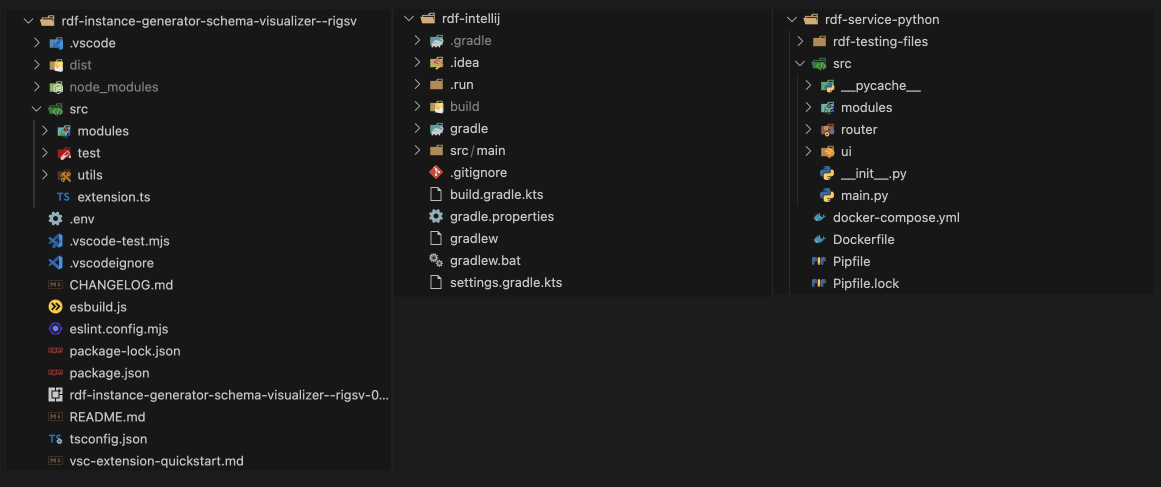
\includegraphics[width=13cm]{folder_structure.png}
  \caption{Project Structure}
  \label{fig:projectstructure}
\end{figure}

The first project is the web service (\texttt{rdf-service-python}), the second is the VSCode extension (\texttt{rdf-instance-generator-schema-visualizer--rigvs}), and the third is the IntelliJ plugin (\texttt{rdf-IntelliJ}).

\section{Implementation of the Web Service\label{sec:webservice}}

\begin{figure}[htb]
    \centering
    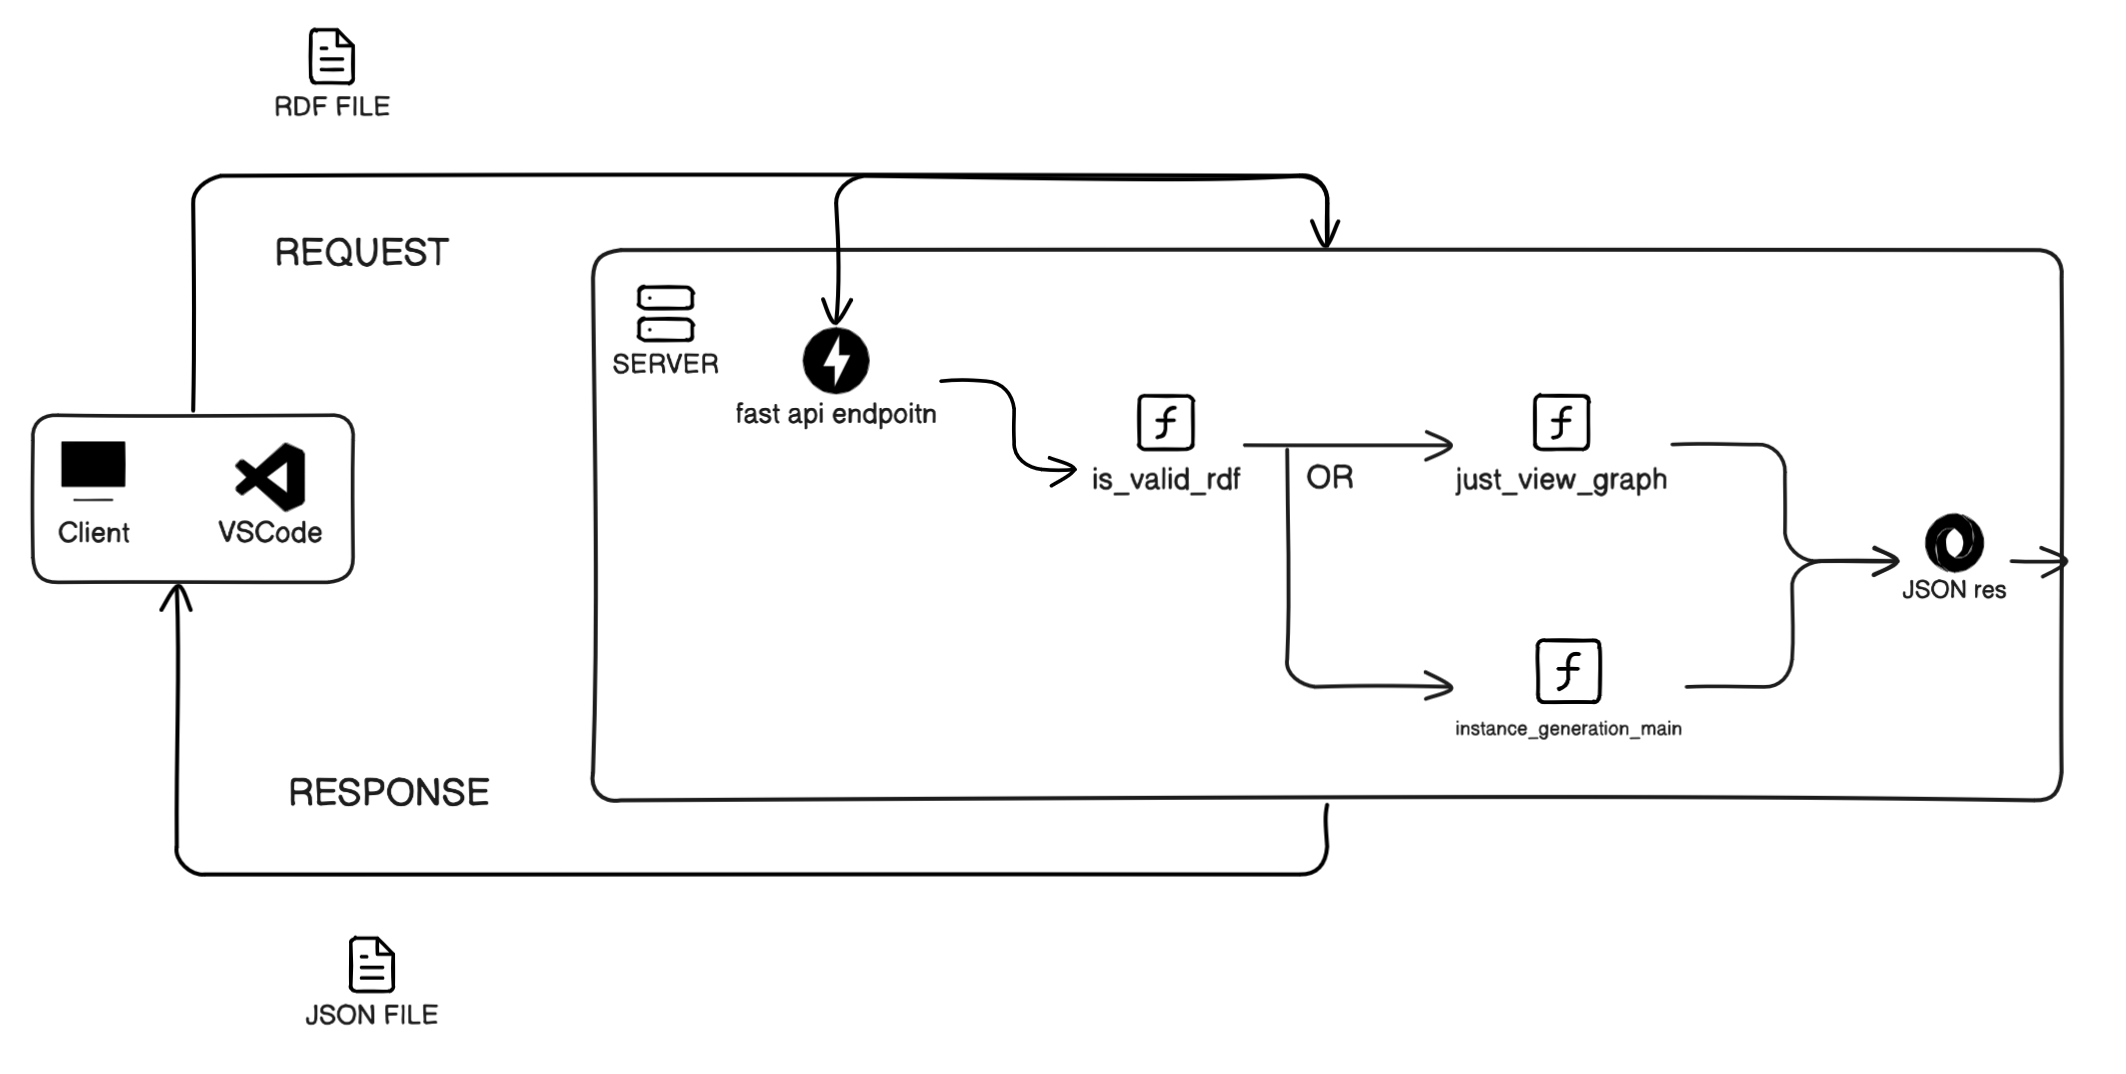
\includegraphics[width=13cm]{server_schema.png}
    \caption{Server Schema}
    \label{fig:serverschema}
\end{figure}

\noindent
The following section details the implementation of the web service and its key components.
\\
\\
\subsection{Server} 
Among the many Python libraries available for creating a REST web service, FastAPI was selected. It is a modern, high-performance web framework for building APIs in Python, based on standard Python type hints \cite{fastapi}.
\\
The first step in setting up the server involved installing FastAPI and its dependencies. After that, initializing the app object (\texttt{app = FastAPI()}) and running the command \texttt{fastapi dev src/main.py} started the server.
\\
\\
The next step was to create the endpoints. In \texttt{src/router/router.py}, the router was initialized with \texttt{router = APIRouter()}, and three endpoints were created: two for the browser client and one for the extensions.
\\
\\
The first endpoint, \texttt{@router.get("/", response\_class=HTMLResponse)}, is used to serve the \texttt{index.html} file to the web browser. This page allows users to upload RDF files (via a POST to the next endpoint), visualize the generated graph, and inspect the RDF file with the newly generated instances.
\\
\\
The second endpoint, \texttt{@router.post("/generate", tags=["users"])}, accepts POST requests from the browser with the RDF file. It returns the necessary data in JSON format.
\\
\\
The final endpoint, \texttt{@router.post("/", response\_class=JSONResponse)}, handles POST requests from the VSCode and IntelliJ extensions. It also returns data in JSON format.

\subsection{RDF Validation} 
When an endpoint receives an RDF file, the first function called is \texttt{is\_valid\_rdf(file)}. This asynchronous function is responsible for validating the incoming RDF file. First, it extracts the file extension and checks whether it exists in a predefined dictionary. If not, an error is returned; otherwise, the process continues.
\\
To verify both syntactic and semantic correctness, the function uses the \texttt{rdflib} library. This library allows parsing and serialization of RDF data, storing RDF triples, accessing SPARQL endpoints, and working with RDF graphs \cite{rdflib}.
\\
The core of this function uses \texttt{Graph.parse()}. If the file is valid, a new RDF graph is generated and returned; otherwise, the function returns \texttt{False}.

\subsection{Graph Generator}
After validating the RDF file, the next step is graph generation. The \texttt{getGraph()} function uses the parsing logic mentioned above to return the graph, the file extension, and the format to the \texttt{just\_view\_graph()} function.
\\
The graph is then serialized into the requested format and into JSON-LD.

\subsection{Instance and Graph Generator}
This is the most important and complex functionality of the entire project. 
Just like in the previous step, the graph, file format, and extension are returned from \texttt{getGraph()}.
A new graph is then initialized. To maintain consistency and readability, all namespace prefixes from the original graph (\texttt{or\_graph}) are copied to the new one.
\\
\\
The RDF graph is then scanned using the \texttt{scan()} function, which extracts classes and properties. First, \texttt{detect\_classes()} retrieves class definitions, then \texttt{detect\_properties()} links properties to their domain and range. This ensures that all indirectly referenced classes are included.
\\
\\
Two generation paths are implemented: instance generation without property search, and with property search.
\\
\\
In RDF vocabularies, classes may be explicitly declared (e.g., \texttt{rdf:type rdfs:Class}) or implicitly referenced via property definitions (e.g., \texttt{rdfs:range schema:Car}).
\\
In the case of generation without property search, the system generates instances for all identified classes—explicit or implicit.
\\
The \texttt{generate\_instance()} function receives the class URI, the new graph, the number of instances, and any defined properties.
\\
\\
If the class URI starts with \texttt{http://www.w3.org/2001/XMLSchema}, it is skipped. Then, two dictionaries are initialized: \texttt{processed\_instances} (to avoid duplicate generation) and \texttt{initialized\_instances} (to track assigned properties).
\\
\\
The function iterates \texttt{N} times to create instances. For each, a new URI is created (e.g., \texttt{ex:Employee\_Instance1}), linked to the class URI, and added to the graph. If an instance has properties, each is processed as follows:
\begin{itemize}
    \item If the value is a URI and maps to a primitive datatype, a literal is generated based on a predefined XSD hashmap.
    \item If the URI refers to another class, the function is called recursively to generate a sub-instance.
    \item If the value is an XSD datatype URI, a default literal is created.
    \item If the value is already a literal, it is directly added.
    \item If the value type is unsupported, an error is raised.
\end{itemize}
Each initialized property is recorded in \texttt{initialized\_instances}. Once all instances are generated, they are returned.

\subsection{Property Search}
If the property search option is enabled, additional steps are required. After class detection, the \texttt{find\_properties()} function retrieves implicitly referenced classes, then uses the \texttt{query()} function to fetch properties from the Linked Open Vocabularies (LOV) endpoint.
\\
\\
The \texttt{query()} function accepts a class term, the number of desired properties, and the ontology to search. It constructs a SPARQL query using \texttt{fetchQuery()} and runs it via \texttt{sparqlwrapper}. The results are filtered, randomized, and mapped to the target class.
\\
\\
The \texttt{find\_properties()} output is passed to \texttt{update\_props()} to enrich the property definitions used in \texttt{generate\_instance()}.
\\
\\
Finally, the new graph is merged with the original RDF graph and returned as a JSON response, along with the file name and its JSON-LD serialization.
\\
\\
\begin{lstlisting}[caption={Main Function for RDF Instance Generation}, label={lst:instance_generation_main}]
	async def instance_generation_main(file, n=2, property_search=False):
		or_graph, format, fileFormatName = await getGraph(file)
	
		if or_graph is None:
			return None
	
		new_instances_graph = Graph()
		for prefix, namespace in or_graph.namespace_manager.namespaces():
			new_instances_graph.namespace_manager.bind(prefix, namespace)
	
		# Detect classes and their properties
		classes = scan(or_graph)
		property_definitions = {
			class_uri: details["properties"]
			for class_uri, details in classes.items()
		}
	
		if property_search == True:
			undeclared_classes_props = find_properties(classes, 1)
			new_property_definitions = update_props(property_definitions, undeclared_classes_props)
	
			for class_uri in classes:
				generate_instance(
					class_uri,
					new_instances_graph,
					num_instances=n,
					property_definitions=new_property_definitions
				)
		else:
			for class_uri in classes:
				generate_instance(
					class_uri,
					new_instances_graph,
					num_instances=n,
					property_definitions=property_definitions
				)
	
		rdf_data = save_to_new_response(or_graph, new_instances_graph, fileFormatName)
		json_dl = rdf_format_json(rdf_data, fileFormatName)
	
		return {
			"data": rdf_data,
			"fileName": f"new_rdf{format}",
			"json_dl": json_dl
		}
	\end{lstlisting}

\section{Implementation of the Browser Application}

The following section describes the implementation of the browser application, focusing on the client-side code.

\begin{figure}[htb]
    \centering
    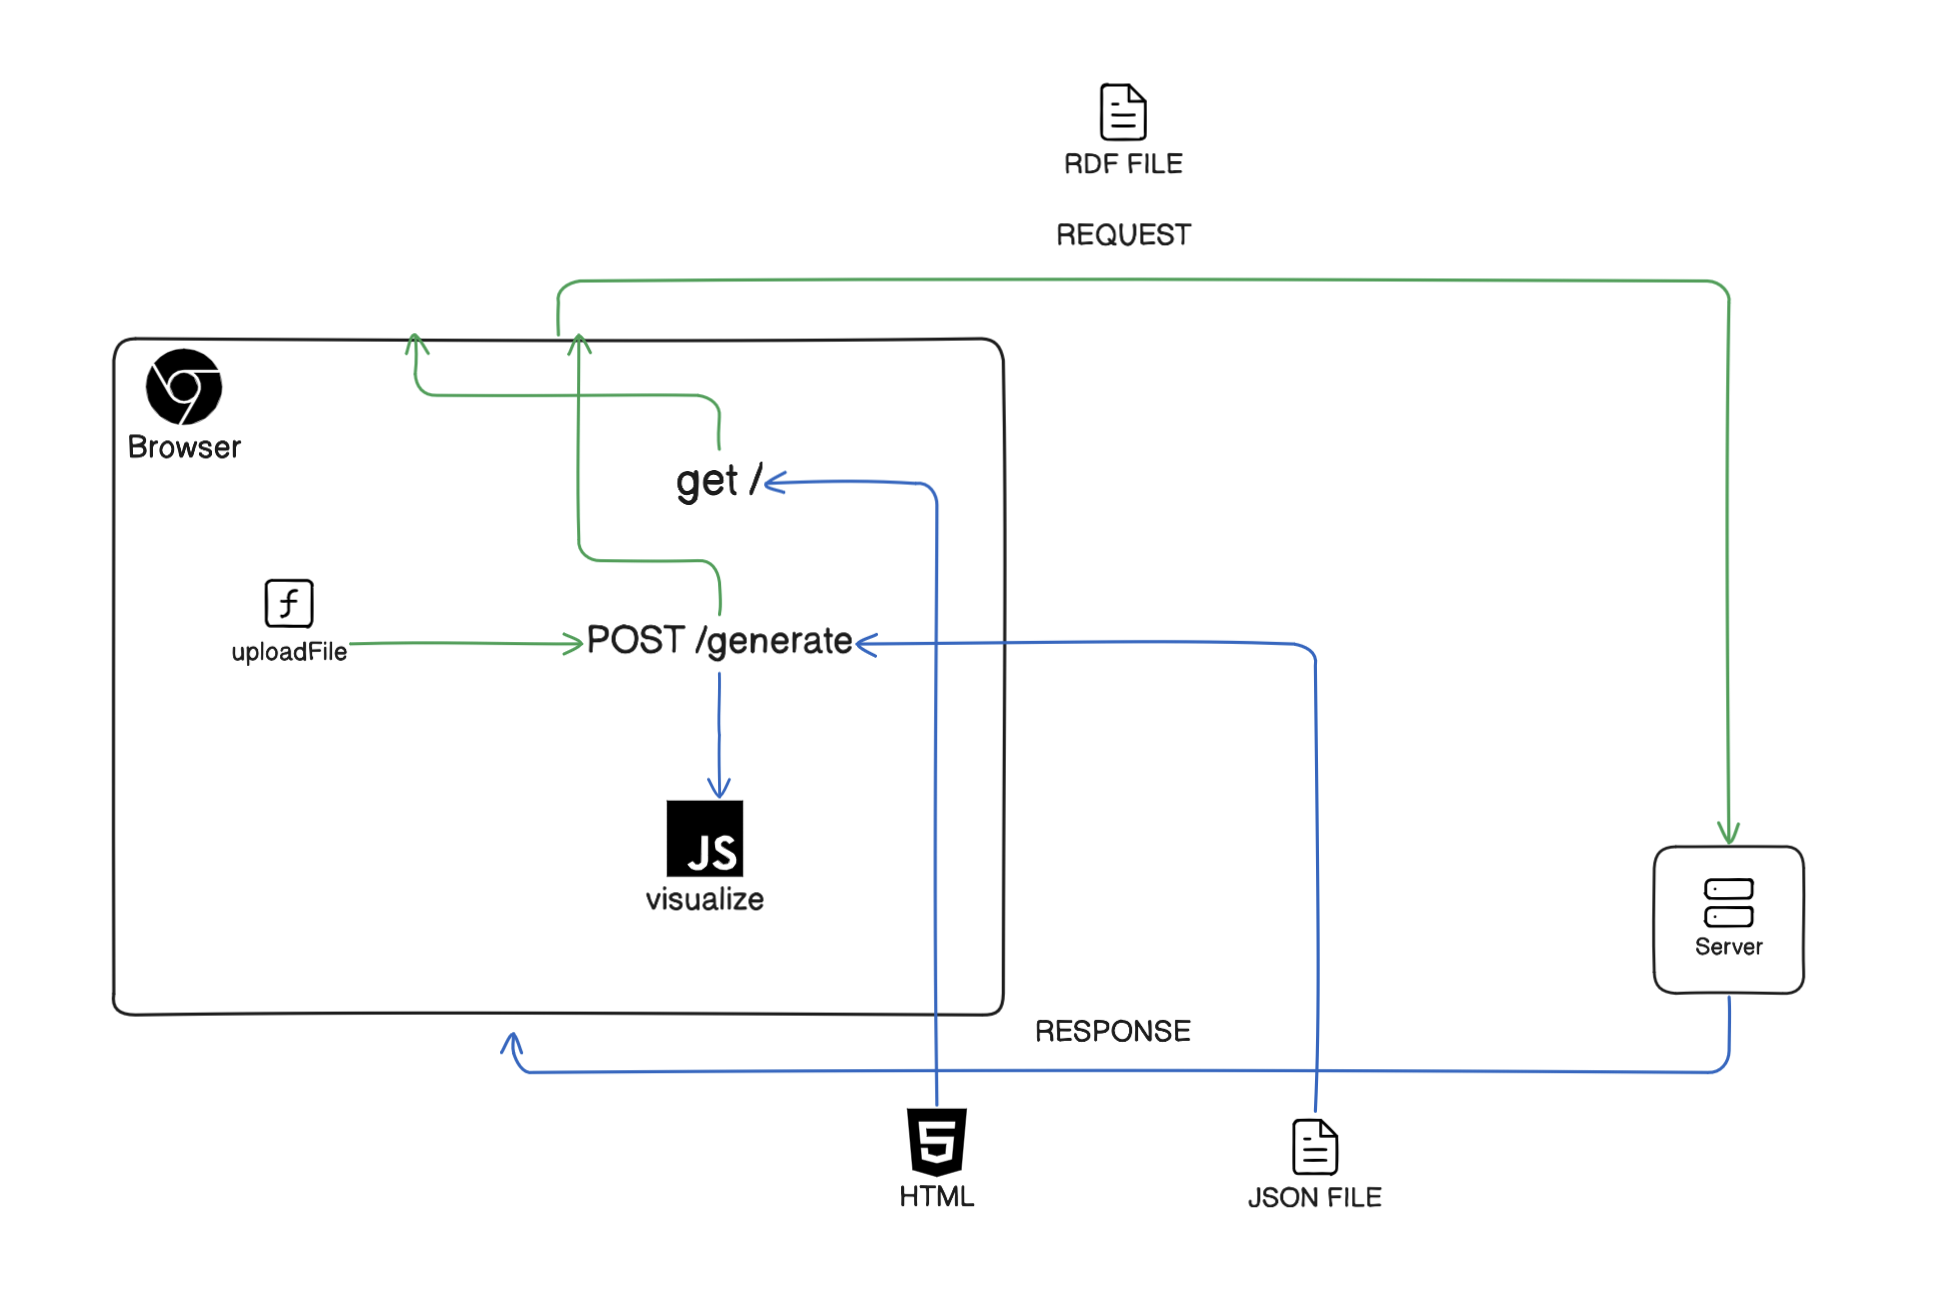
\includegraphics[width=13cm]{dataflow-browser-rdf-request.png}
    \caption{Web extension}
    \label{fig:dataflow-browser-rdf-request}
\end{figure}

\subsection{The Fetch}
When users want to use the RDF Instance Generator and Visualizer, the quickest way is through a web browser. 
\\
By accessing the server’s default route (\texttt{/}), an HTML page is returned. This page allows users to upload an RDF file to the server (\texttt{/generate} route). 
Upon a successful upload, users can inspect the new RDF file and view the generated JSON-LD graph using the \texttt{vis.js} library.
\\
The following describes the pipeline for converting JSON-LD into an interactive RDF graph.

\subsection{Graph Rendering}
When the \texttt{index.html} file is rendered, it loads two main JavaScript files: \texttt{uploader.js} and \texttt{visualizer.js}.  
The first script creates a web component called \texttt{TurtleFileUploader}, which enables users to upload files and send POST requests.  
Upon receiving a successful response, it injects the \texttt{json\_ld} data into the custom \texttt{rdf-visualizer} as a \texttt{jsondata} attribute.  
Additionally, the new RDF file (\texttt{res.data}) is attached to the DOM so the user can inspect and download it.
\\
\\
\begin{lstlisting}[caption={\texttt{TurtleFileUploader} component}, label={lst:turtle-file-uploader}, language=JavaScript]
class TurtleFileUploader extends HTMLElement {
  constructor() { ... }

  connectedCallback() { ... }

  async uploadFile(edit = false, search = false) {
    const fileInput = this.shadowRoot.getElementById("fileInput");
    const responseDiv = this.shadowRoot.getElementById("response");
    const rdfVisualizer = document.getElementById("rdfVisualizer");
    const n = this.shadowRoot.getElementById("n").value;

    if (fileInput.files.length === 0) { ... }

    if (search && n > 3) { ... }

    const formData = new FormData();
    formData.append("file", fileInput.files[0]);

    try {
      const response = await fetch(`/generate?n=${n}&edit=${edit}&property_search=${search}`, {
        method: "POST",
        body: formData
      });

      if (!response.ok) throw new Error(`HTTP error! Status: ${response.status}`);

      const res = await response.json();
      responseDiv.innerText = res.data;

      const blob = new Blob([res.data]);
      const url = URL.createObjectURL(blob);
      const a = document.createElement("a");
      a.href = url;
      a.download = res.fileName;
      a.innerText = `Download ${res.fileName}`;
      a.style.display = "block";
      responseDiv.appendChild(a);

      rdfVisualizer.setAttribute("jsondata", res.json_dl);
    } catch (error) {
      responseDiv.innerHTML = "Error: " + error.message;
    }
  }
}

customElements.define('turtle-file-uploader', TurtleFileUploader);
\end{lstlisting}

The second script defines the \texttt{rdf-visualizer} component. This component listens for the \texttt{jsondata} attribute and triggers a parser function to safely deserialize the data.  
To ensure consistent rendering, the data is normalized into an array of RDF subject objects, each containing an ID, type, and property-value pairs.
\\
\\
The core conversion from RDF semantics to network-compatible format is handled by the \texttt{processJsonLd} function.  
Each RDF subject is transformed into a graph node and classified as:
\begin{itemize}
    \item \textbf{Class} (\texttt{rdfs:Class}) – shown as orange boxes
    \item \textbf{Property} (\texttt{rdf:Property}) – shown as green-yellow diamonds
    \item \textbf{Instance} (URI-based) – shown as blue dots
    \item \textbf{Literal} – shown as yellow boxes
\end{itemize}
\bigskip 
\begin{lstlisting}[caption={\texttt{processJsonLd} function used for graph construction}, label={lst:rdf-visualizer}, language=JavaScript]
function processJsonLd(data, dynamicPrefixes) {
  const nodesMap = {};
  const edges = [];
  let literalCounter = 0;

  data.forEach(item => {
    const subjectId = item['@id'];
    let nodeType = 'instance';

    if (item['@type']) {
      const types = Array.isArray(item['@type']) ? item['@type'] : [item['@type']];
      if (types.includes("...#Class")) nodeType = 'class';
      else if (types.includes("...#Property")) nodeType = 'property';
    }

    if (!nodesMap[subjectId]) {
      let label = item["...#label"] ? item["...#label"][0]["@value"] : shorten(subjectId, dynamicPrefixes);
      let shape = nodeType === 'class' ? 'box' : nodeType === 'property' ? 'diamond' : 'dot';
      let color = nodeType === 'class' ? '#FFA500' : nodeType === 'property' ? '#ADFF2F' : '#97C2FC';
      nodesMap[subjectId] = { id: subjectId, label, shape, color, baseColor: color, nodeType, font: { color: "#000000" } };
    }

    if (item['@type']) {
      types.forEach(t => {
        let typeId = typeof t === 'string' ? t : t['@id'];
        if (typeId && !nodesMap[typeId]) {
          nodesMap[typeId] = { id: typeId, label: shorten(typeId, dynamicPrefixes), shape: 'box', color: '#FFA500', ... };
        }
        edges.push({ from: subjectId, to: typeId, label: shorten("...#type", dynamicPrefixes), dashes: true, color: { color: '#000' } });
      });
    }

    Object.keys(item).forEach(prop => {
      if (prop === '@id' || prop === '@type') return;
      item[prop].forEach(val => {
        if (val['@id']) {
          if (!nodesMap[val['@id']]) nodesMap[val['@id']] = { id: val['@id'], label: shorten(val['@id'], dynamicPrefixes), shape: 'dot', ... };
          edges.push({ from: subjectId, to: val['@id'], label: shorten(prop, dynamicPrefixes), arrows: 'to', ... });
        } else if (val['@value']) {
          const literalId = `literal_${literalCounter++}`;
          nodesMap[literalId] = { id: literalId, label: String(val['@value']), shape: 'box', color: '#FFD700', ... };
          edges.push({ from: subjectId, to: literalId, label: shorten(prop, dynamicPrefixes), arrows: 'to', ... });
        }
      });
    });
  });

  return { nodes: Object.values(nodesMap), edges };
}
\end{lstlisting}

Each RDF triple is mapped as an edge between a subject and an object, labeled by the predicate.  
Type relationships (i.e., \texttt{rdf:type}) are visualized using dashed lines to distinguish them from regular property connections.
\\
\\
After defining the nodes and edges, the data is loaded into a \texttt{vis-network} object.  
The layout engine distributes the graph nodes automatically, and a stabilization process improves readability.  
To enhance user experience, when a node is clicked, all non-neighboring nodes are blurred out to focus attention.

\section{Implementation of the Visual Studio Code Extension}    

Visual Studio Code, originally intended as a lightweight source code editor, has evolved into a fully functional IDE thanks to its extensive plugin ecosystem.
\\
Since VSCode is built on top of Electron—a framework for building desktop applications using web technologies—it is possible to build extensions using familiar web tools (HTML, CSS, JavaScript).
\\
This extension is developed using the Visual Studio Code Extension API, which provides interfaces and classes for interacting with the editor’s core features.
\\
The following section describes the implementation of the VSCode extension and its key features.

\begin{figure}[htb]
    \centering
    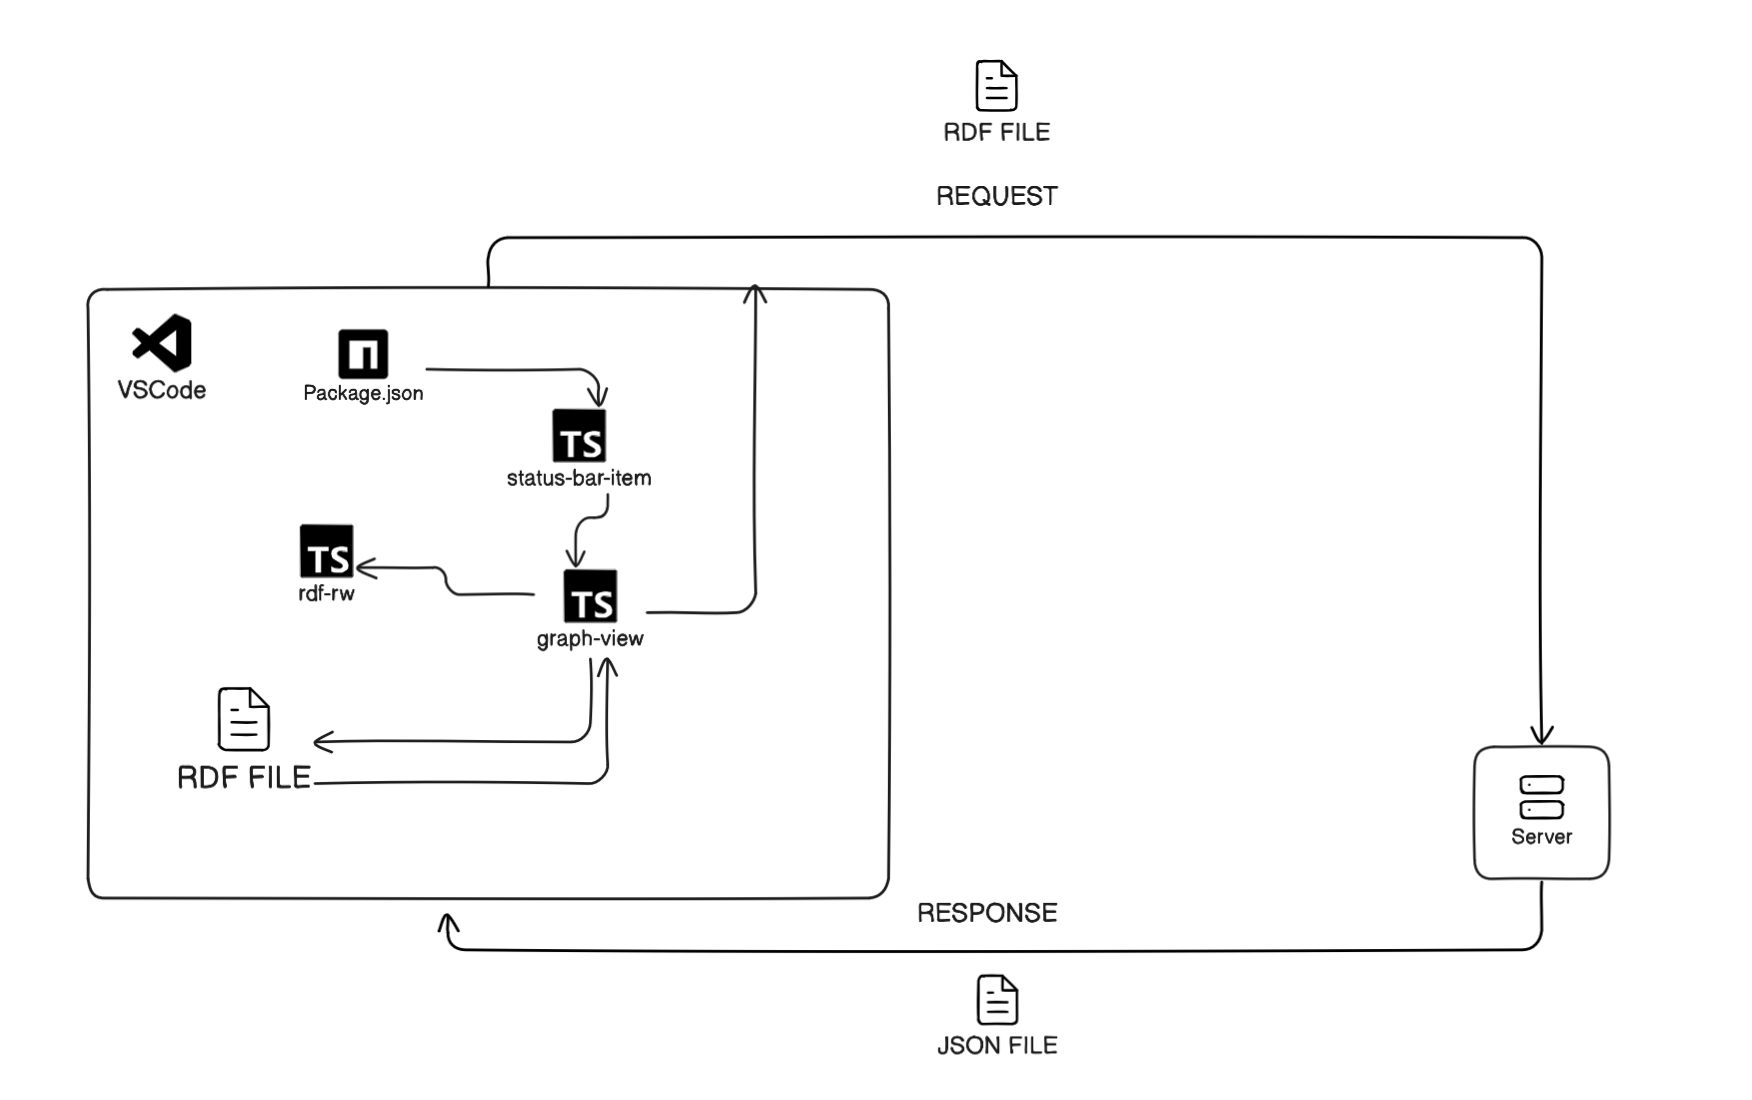
\includegraphics[width=13cm]{dataflow-vscode-extension.png}
    \caption{VSCode extension}
    \label{fig:vscode-extension}
\end{figure}

\subsection{Commands Architecture}
Commands trigger actions in Visual Studio Code. In this project, commands are used by the RIGVS extension to expose the following features to users:
\begin{itemize}
    \item \texttt{extension.viewGraph} – View RDF graph
    \item \texttt{extension.runGraph} – Generate instances and view graph
    \item \texttt{extension.searchProperty} – Generate instances with properties and view graph
\end{itemize}
\bigskip 
\begin{lstlisting}[caption={package.json commands declaration}, label={lst:commands-declaration}, language=JavaScript]
...
"commands": [
  {
    "command": "extension.runGraph",
    "title": "RIGSV generate instance & view graph"
  },
  {
    "command": "extension.searchProperty",
    "title": "RIGSV generate instance with properties"
  },
  {
    "command": "extension.openMenu",
    "title": "RIGSV Options"
  },
  {
    "command": "extension.settings",
    "title": "RIGSV settings"
  },
  {
    "command": "extension.viewGraph",
    "title": "RIGSV view graph"
  },
  {
    "command": "extension.editRDF",
    "title": "RIGSV edit RDF"
  }
],
...
\end{lstlisting}

All commands in VSCode can be executed using \texttt{cmd + shift + p}. After opening the input dialog, users can run any command by typing its title and pressing enter.
\\
\\
The first command, \texttt{extension.viewGraph}, opens a WebView inside the VSCode workspace. This WebView displays the graph returned by the server.
\\
Currently, this command only works while an RDF file is focused in the editor. When executed, it creates a new panel via \texttt{vscode.window.createWebviewPanel}, with scripts enabled and placed beside the editor window. The \texttt{getWebviewContent} function is then called.
\\
\\
This function extracts the RDF content from the focused file using \texttt{getRDFContent} and sends it to the server via \texttt{sendRDFContent}. Then it injects static URLs for the necessary scripts (\texttt{visualizer.js} and \texttt{uploader.js}) into the HTML content.
\\
\\
Because VSCode WebViews operate in a sandboxed environment, Content Security Policies (CSP) restrict access to external scripts and styles. To work around this, a meta tag is added to the HTML head:
\\
\\
\texttt{<meta http-equiv="Content-Security-Policy" content="\$\{csp\}">}
\\
\\
After the content is prepared, it is rendered inside the WebView panel. The page also listens for two specific button clicks: \texttt{editButton} and \texttt{exportGraph}.
\\
Clicking \texttt{editButton} triggers the command \texttt{extension.editRDF}, which opens the new RDF graph in the editor using the original RDF format.
\\
The \texttt{extension.exportGraph} command allows exporting the rendered graph as a PNG image.
\\
\\
The second command, \texttt{extension.runGraph}, performs the same functions but adds a pop-up input that asks the user for the number of instances to generate.
\\
The final command, \texttt{extension.searchProperty}, behaves like \texttt{runGraph} but includes the additional property search functionality.

\begin{lstlisting}[caption={openWebView}, label={lst:open-web-view}, language=JavaScript]
export function openWebView(context: vscode.ExtensionContext) {
  const viewGraph = vscode.commands.registerCommand(
    "extension.viewGraph",
    async () => {
      vscode.window.showInformationMessage("Graph view is loaded");

      let panel = vscode.window.createWebviewPanel(
        "rdfVisualizer",
        "RDF Visualizer",
        vscode.ViewColumn.Beside,
        {
          enableScripts: true,
          retainContextWhenHidden: false,
        }
      );

      if (envConfig.serviceEndpoint) {
        const htmlContent = await getWebviewContent(
          panel.webview,
          envConfig.serviceEndpoint,
          true
        );
        panel.webview.html = htmlContent;
      }

      panel.webview.onDidReceiveMessage(
        async (message) => {
          if (message.command === "editRDF") {
            vscode.commands.executeCommand("extension.editRDF");
          }
        },
        undefined,
        context.subscriptions
      );
      exportGraph(panel)
    }
  );
  const runGraph = vscode.commands.registerCommand(...)
  const searchProperty = vscode.commands.registerCommand(...)
  const editRDFCommand = vscode.commands.registerCommand(...)
  ...
}
\end{lstlisting}

Currently, these commands can only be used while an RDF file is focused in the editor.
\\
To simplify access, a quick-access menu button has been added to the bottom-right corner of the VSCode window. Clicking the button opens a modal that allows users to select between the three available commands.
\section{Implementation of the IntelliJ IDEA plugin}    

The following section describes the implementation of the IntelliJ IDEA plugin and showcases its key feature.

\begin{figure}[htb]
    \centering
    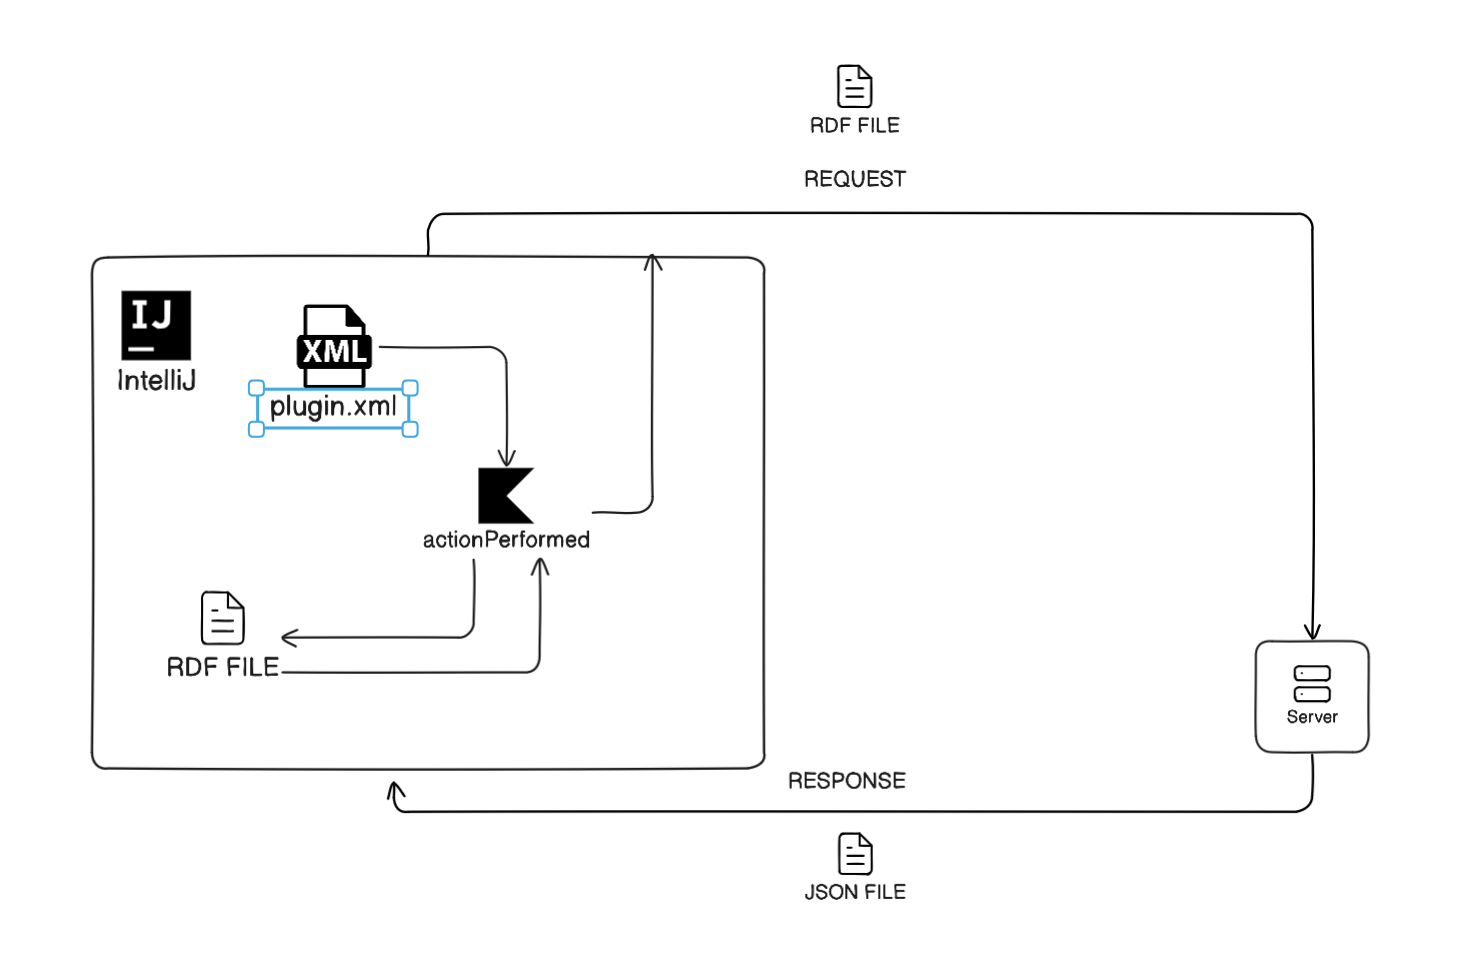
\includegraphics[width=13cm]{dataflow-intellij-extension.png}
    \caption{IntelliJ Extension}
    \label{fig:intellijextension}
\end{figure}

Similar to the VSCode extension, the goal of the IntelliJ IDEA plugin is to provide a user-friendly interface for generating RDF instances and visualizing them in a side panel as a graph.
\\
This extension, developed primarily to demonstrate the flexibility of the tool’s distributed architecture, currently implements only the feature responsible for rendering RDF graphs in a side panel.
\\
\\
The plugin is developed using the Kotlin programming language, the Gradle plugin manager, and the JetBrains Plugin DevKit.
\\
Like in VSCode, the IntelliJ plugin defines \textbf{actions} (comparable to VSCode’s \texttt{commands}) that execute specific functions in response to user interactions.

\begin{lstlisting}[caption={IntelliJ Actions}, label={lst:actions}, language=xml]
<?xml version="1.0" encoding="UTF-8"?>
<idea-plugin>
    <id>com.example.rdf</id>
    <name>RDF Visualizer</name>
    <vendor>Wesley G. Obi</vendor>
    <description>Visualizing RDF Files Graphically Using an External Python Service</description>

    <depends>com.intellij.modules.platform</depends>

    <actions>
        <action id="RDFVisualizer.Convert"
                class="com.example.rdf.RDFVisualizerAction"
                text="Visualize RDF"
                description="Converts the current RDF file into a graphical visualization">
            <add-to-group group-id="EditorPopupMenu" anchor="last"/>
        </action>
    </actions>
</idea-plugin>
\end{lstlisting}

When a user right-clicks on an RDF file, the \textbf{Visualize RDF} action appears in the context menu.

\begin{figure}[htb]
    \centering
    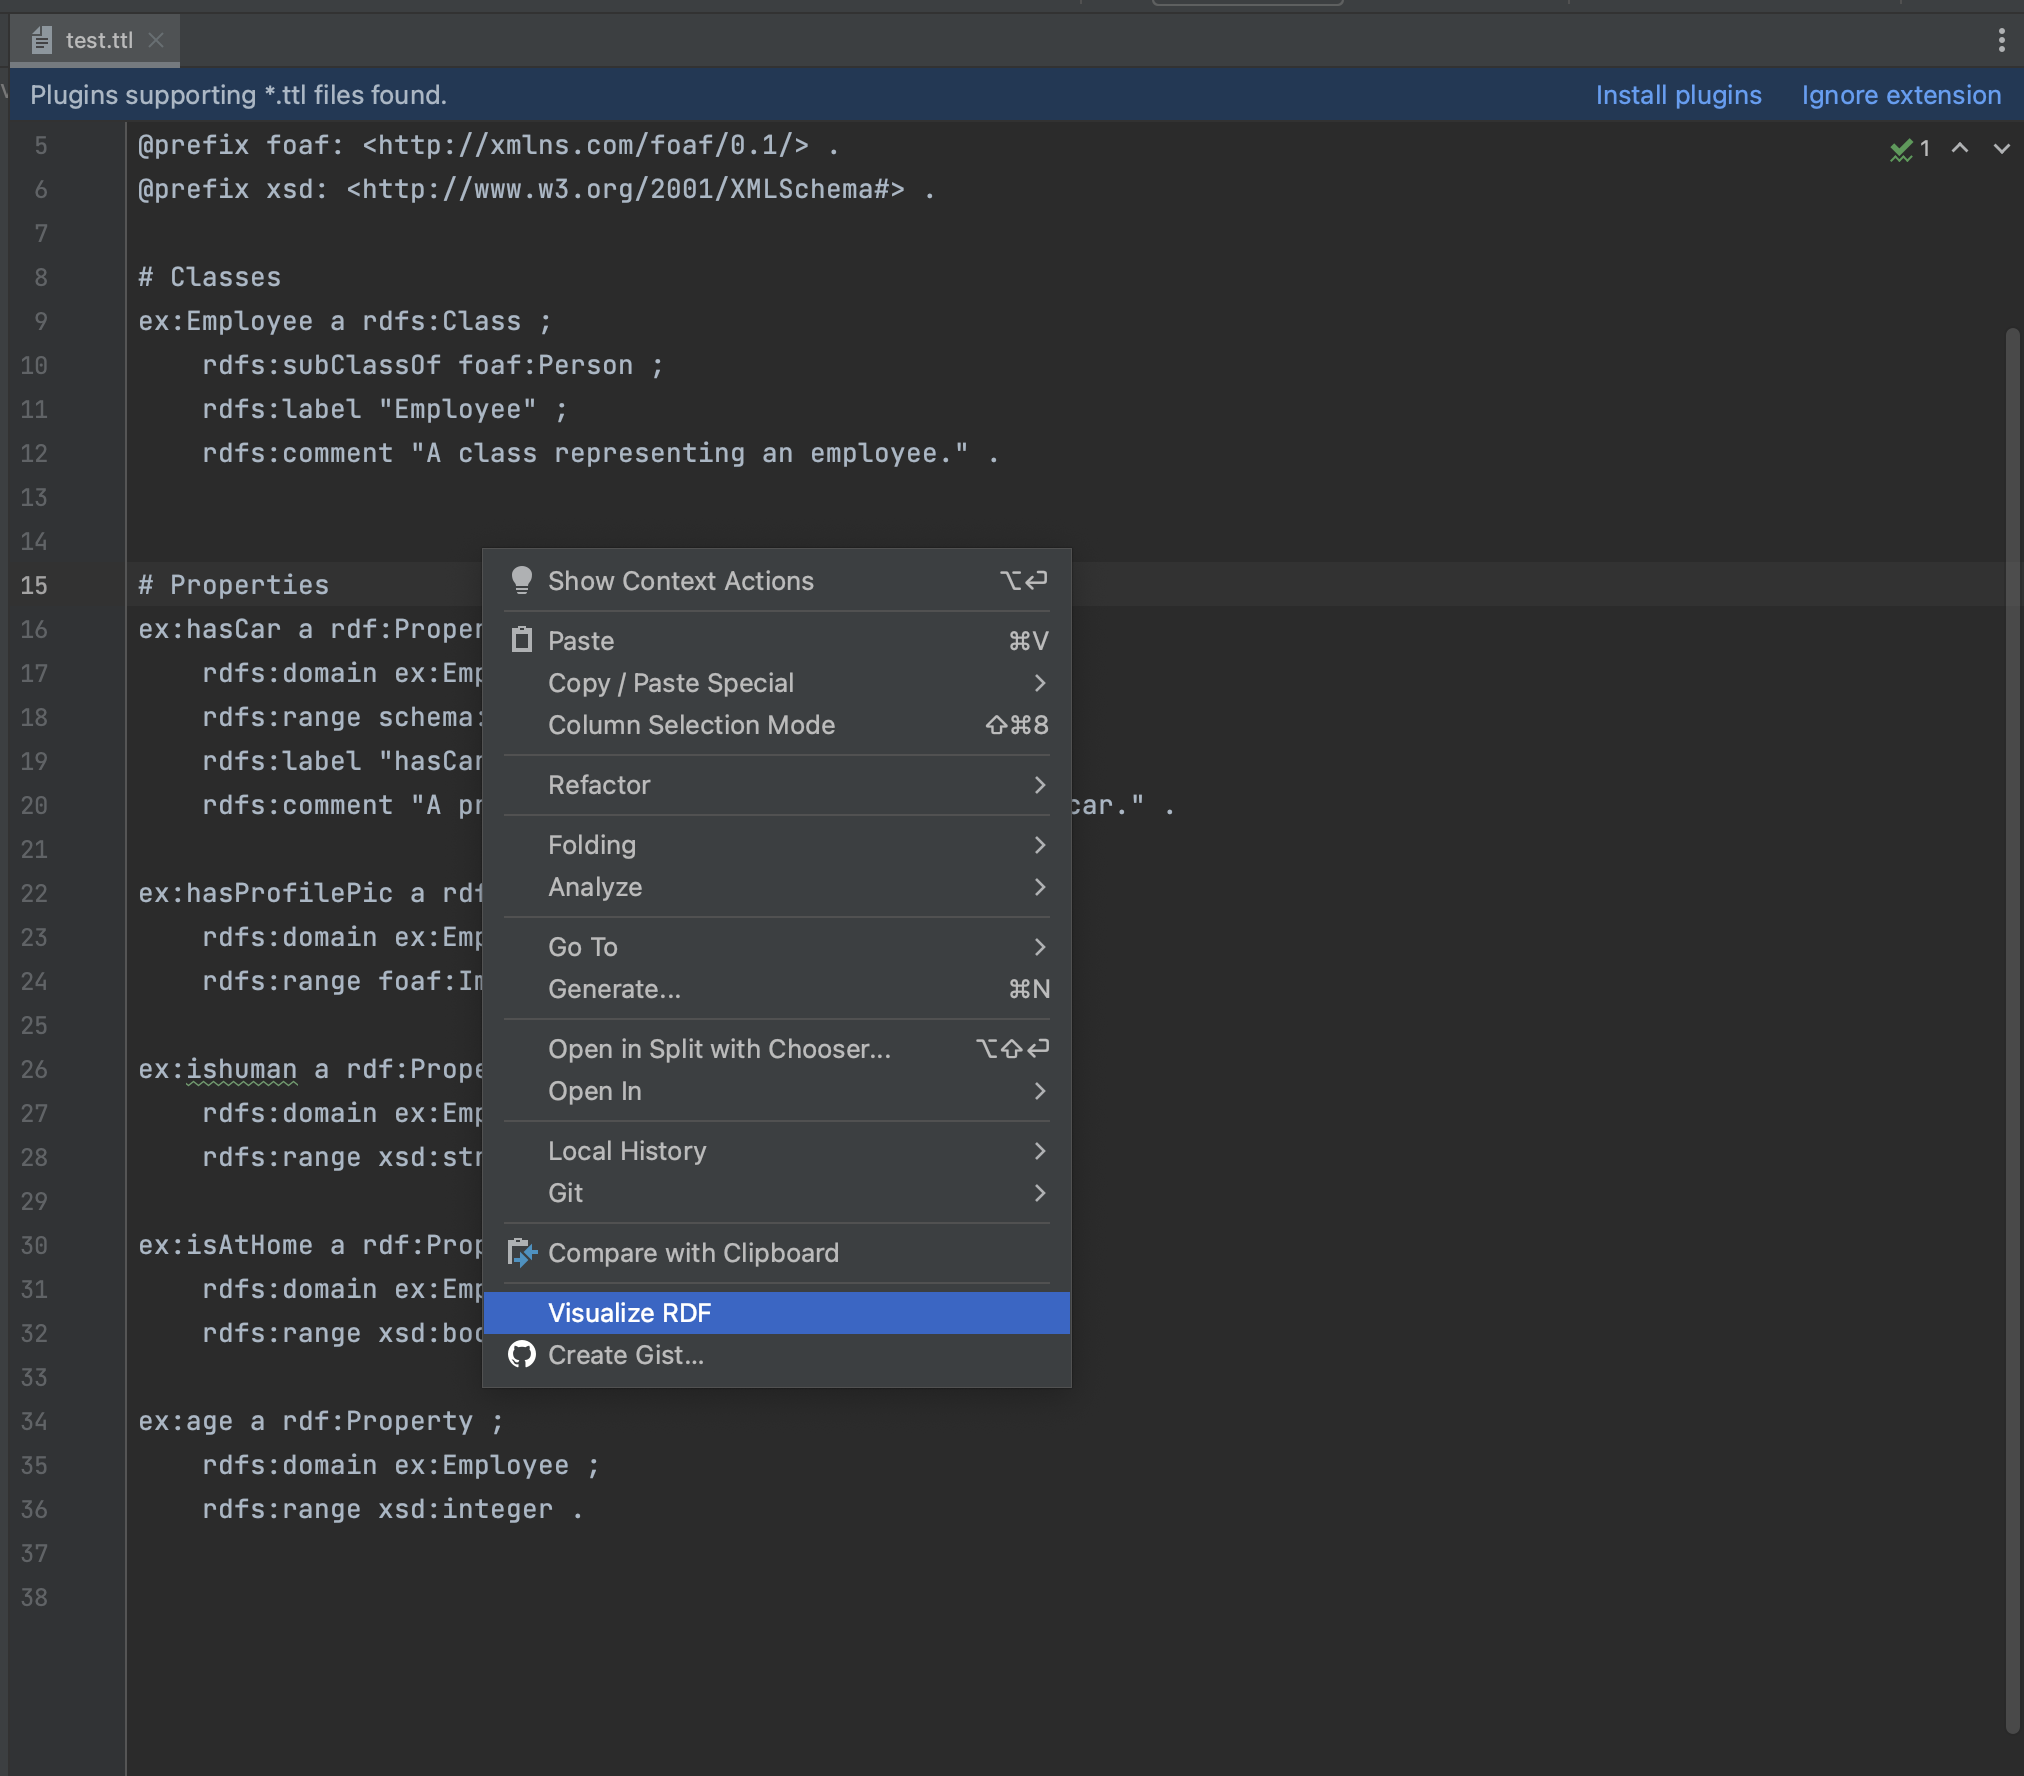
\includegraphics[width=14cm]{actioncallinintellij.png}
    \caption{Action call in IntelliJ}
    \label{fig:actioncallinintellija}
\end{figure}

By simply clicking on it, the action is triggered and executes the \texttt{actionPerformed} function.
\\
This function extracts the RDF schema from the currently focused file, wraps it in a \texttt{formData} object, and sends it to the Python server.
\\
The response is passed to the \texttt{showGraphViewer} function, which renders the graph in a side panel.
\\
As in the VSCode extension, the HTML content is adjusted to bypass CSP restrictions, ensuring that external resources (scripts and styles) can be loaded and rendered properly inside the IntelliJ WebView.

\begin{lstlisting}[caption={Render graph in WebView in IntelliJ}, label={lst:open-web-view-intellij}, language=Java]
override fun actionPerformed(e: AnActionEvent) {
    ...
    val formData = MultipartBody.Builder()
        .setType(MultipartBody.FORM)
        .addFormDataPart("fileUpload", file.name, requestBody)
        .build()

    val request = Request.Builder()
        .url("http://localhost:8000/")
        .post(formData)
        .build()

    val client = OkHttpClient()

    try {
        val response = client.newCall(request).execute()
        if (response.isSuccessful) {
            val jsonResponse = response.body?.string() ?: throw Exception("Empty response body")
            val responseBody: ServerResponse = Json.decodeFromString(jsonResponse)

            showGraphViewer(project, responseBody.content)
        } else { ... }
        ...
    }
}
\end{lstlisting}

\section{Documentation and Deployment Architecture\label{sec:docu}}

The documentation for this project is available in the GitHub repository in the \texttt{README.md} file.  
It provides two types of installation instructions: Developer installation and User installation.
\\
\\
For developers, the setup involves installing the required programming languages, runtimes, and dependencies (e.g., Python, Node.js, pip, npm).  
Additionally, they must start the Python server and load the extension inside the VSCode development environment.
\\
\\
For end users, the installation process is significantly simpler.  
The repository already includes a pre-built version of the VSCode extension, which can be installed like any other VSCode extension.
\\
\\
To ensure compatibility across different systems and avoid requiring users to manually install any development tools, the web service has been containerized using Docker.  
This allows users to run the system by simply installing Docker Desktop, without needing to configure environments or install dependencies manually.